% !TeX root = ../main.tex

\chapter{相关技术和理论概述}\label{equations}
本文主要研究的内容是神经辐射场在新视图合成上的加速,因此本章首先主要介绍神经三维形状表示法,新视图合成和基于图像的渲染方法。随着深度学习的发展,当今效果最佳的新视图合成算法都是基于深度学习的,因此接下来会概述深度学习的原理和发展状况,并重要介绍基于深度学习的神经辐射场的立体渲染方法。最后介绍一下查询表的概念,以及查询表在逐点网络上的加速应用,为本文方法的展开做好铺垫。

\section{神经三维形状表示法}
三维物体的形状表示有多种方法,例如传统的基于点,基于网格,基于体素的方法。此外,还有最新的基于深度学习的三维形状表示方法,下面对以上四种表示方法分别进行阐述。

\subsection{基于点的表示方法} 
基于点的方法一般指的是点云(如图~\ref{fig:stanfordRabbit} 所示的第一个)这种表示,点云是指空间中一组点的集合,每一个点都包含 X,Y,Z 三个坐标。它是一种轻量级的三维表示方式,与匹配许多传感器(例如雷达,深度相机)提供的原始数据非常匹配,因此非常适合应用在三维学习技术上。例如 PointNet\cite{qi2017pointnet,qi2017pointnet++} 这篇非常经典的点云工作,使用最大池化操作来提取全局特征,之后这项技术被广泛用作点生成网络\cite{yang2017foldingnet,achlioptas2018learning}的编码器。此后点云学习方面又涌入了大量的 PointNet 风格的相关工作。然而,点云这种表示方法有着很明确的限制,它们不适用于描述拓扑结构,同时也不适合用以生成紧致的表面。

\subsection{基于网格的表示方法}
许多方法使用预定义模板的网格,它们表征了一系列相似形状的物体,例如可变形的人体部位,其中一些模型\cite{2017Deformable}展示了高保真的形状生成结果。其他的最近工作\cite{baque2018geodesic}使用多边形立方体映射\cite{tarini2004polycube}对形状进行优化。虽然模板网格的使用很方便,并且自然地提供了三维对应,但它只能对具有固定网格拓扑的形状进行建模。其他基于网格的方法使用已有的\cite{sinha2016deep,maron2017convolutional}或者学习的\cite{groueix2018papier,ben2018multi}参数化技术通过二维平面来描述三维曲面。这种表示的质量取决于参数化算法,这些算法通常对输入网格质量和切割策略非常敏感。为了解决这个问题,最近的数据驱动方法\cite{yang2017foldingnet}学习深度网络的参数化任务。然而,他们报告说需要多个平面来描述复杂的拓扑,但是生成的曲面片没有缝合,即生成的形状没有闭合。为了生成闭合网格,可以使用球体参数化\cite{groueix2018papier,ben2018multi},但生成的形状仅限于拓扑球体。其他与网格学习相关的工作建议对网格\cite{defferrard2016convolutional,verma2018feastnet}或一般图\cite{bruna2013spectral}使用新的卷积和池化运算。网格表示三维物体的直观感受如图~\ref{fig:stanfordRabbit} 所示。

\subsection{基于体素的表示方法}
在三维计算机图形学上,体素代表了三维空间中规则格点所对应的值。与二维位图中的像素一样,体素本身通常不使用其值显式编码其位置(即坐标)。取而代之的是,渲染系统根据其相对于其他体素的位置(即其在构成单个体积图像的数据结构中的位置)来推断体素的位置。体素算是像素由二维空间直接推广到三维空间,有着不少共性。基于体素的学习方法中最直接的变体就是占据栅格。但是由于计算和内存开销呈三次方的增长趋势,因此当前的方法只能处理较低分辨率的情况。因此,基于体素的方法\cite{20153D,Choy20163D}无法保留精细的形状细节,由如图~\ref{fig:stanfordRabbit} 所示的第三个图就能明确这一点,此外,体素在视觉上显示与高保真度形状有显著差异,因为渲染时法线不平滑。基于八叉树\cite{Tatarchenko2017Octree,riegler2017octnet,hane2017hierarchical}的方法一定程度上减轻了稠密体素方法的计算和内存限制,但是提升后的分辨率依然没有产生很好的视觉响应。

\begin{figure}[t]
  \centering
  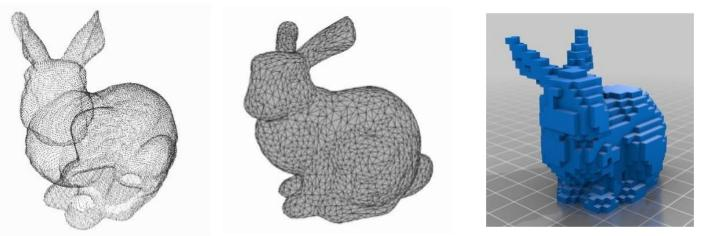
\includegraphics[width=0.9\linewidth]{stanfordRabbit.jpg}
  \caption{三种传统的三维表示方式(点云,网格,体素)}
  \label{fig:stanfordRabbit}
\end{figure}

\subsection{基于深度学习的表示方法}
计算机视觉中最近一个有前景的方向是用多层感知机 MLP 的权值编码对象和场景,MLP 直接从三维空间位置映射到形状的隐式表示,例如该位置的有符号距离\cite{curless1996volumetric},如图~\ref{fig:sdf} 所示是有符号距离函数 (Signed Distance Fuction, SDF)在三维表示上的应用。然而,这些方法到目前为止还无法再现具有复杂几何体的真实场景,其保真度与使用离散表示(如三角形网格或体素网格)表示场景的技术相同。

最近的工作通过优化将 xyz 坐标映射到 SDF 函数\cite{jiang2020local,park2019deepsdf,chabra2020deep}或占据域\cite{genova2020local,mescheder2019occupancy}的深度网络,研究了连续三维形状作为水平集的这种隐式表示。然而,这些模型受到三维几何体 ground truth 的需求的限制,这些几何体通常是从合成的三维形状数据集(例如如 ShapeNet\cite{chang2015shapenet} )获得的。随后的工作通过构造可微的渲染函数,使得神经隐式形状表示仅使用 2D 图像进行优化,从而放宽了对三维形状 ground truth 的要求。Niemeyer 等人\cite{niemeyer2020differentiable}将曲面表示为 3D 占据场,并使用数值方法找到每条光线的曲面交点,然后使用隐式微分计算精确导数。每个光线相交位置都作为神经 3D 纹理场的输入,该纹理场预测该点的颜色。Sitzmann 等人\cite{sitzmann2019scene}使用了一种不太直接的神经 3D 表示法,只需在每个连续的 3D 坐标上输出一个特征向量和 RGB 颜色,并提出了一种可微绘制函数,该函数由一个沿每条射线行进的递归神经网络组成,以确定曲面的位置。

\begin{figure}[t]
  \centering
  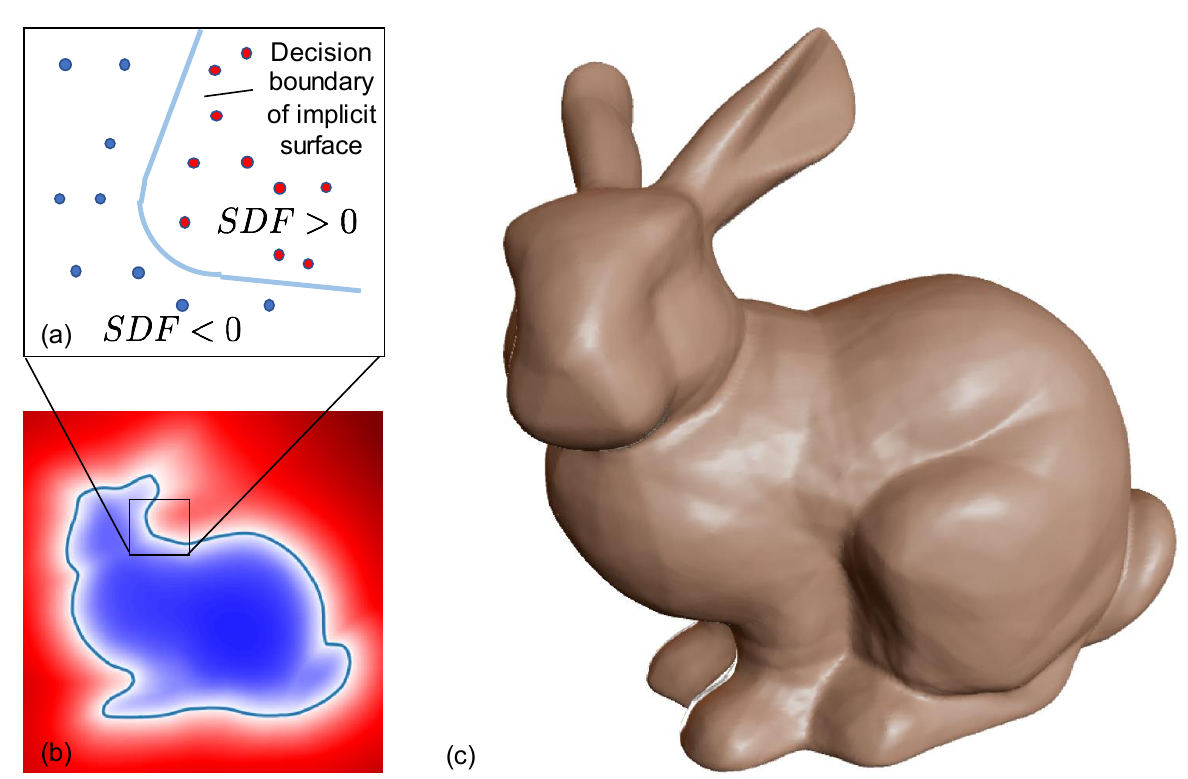
\includegraphics[width=0.8\linewidth]{sdf.png}
  \caption{SDF 函数表示法应用于斯坦福兔子,图片来自于 DeepSDF\cite{park2019deepsdf}。}
  \label{fig:sdf}
\end{figure}

\section{新视图合成和基于图像的渲染}
新视图合成在计算机视觉与计算机图形学这样的交叉领域上是一个长期的问题。所谓新视图合成指的是给定一系列(或者单张)已知相机位姿的视图,由这些视图合成出未知位姿的视图。新视图合成的过程如图~\ref{fig:novelviewsynthesis} 所示。对于给定稀疏视角采样的新视角合成问题,计算机视觉和图形学社区在从观测到的图像中预测传统几何表示的问题上取得了很多进展。一类流行的方法是使用具有要么漫反射\cite{Waechter2014Let}的,要么依赖视角\cite{debevec1996modeling, wood2000surface}的外观的那些 mesh-based(基于网格) 的场景表示。可微分的光栅化器\cite{loper2014opendr,chen2019learning,genova2018unsupervised,liu2019soft}或路径跟踪器\cite{li2018differentiable,nimier2019mitsuba}可以直接通过使用梯度下降法来优化再现一组输入图像的网格表示。然而,基于图像重投影的网格梯度下降的优化是十分困难的,可能是由于局部极小值或 loss 的调整不佳所致。此外,这种策略\cite{li2018differentiable}要求在优化之前提供具有固定拓扑的模板网格作为初始化,这通常对于不受约束的真实场景是不可用的。

另一类方法使用体积表示法来解决从一组输入 RGB 图像中进行高质量逼真的视图合成的任务。体积表示法是能够真实地表达复杂的形状和物体,非常适合基于梯度的优化,比基于网格的方法产生的视觉干扰更少。早期的体积方法\cite{kutulakos2000theory,szeliski1998stereo}使用观察到的图像直接为体素网格着色。最近,几种方法\cite{flynn2019deepview,mildenhall2019local,srinivasan2019pushing,zhou2018stereo}使用了多个场景的大型数据集来训练深层网络,这些深层网络从一组输入图像中预测采样的体积表示,然后使用其中一种 alpha 合成\cite{porter1984compositing}或沿光线学习的合成,以在测试时渲染新视图。其他工作需要针对每个特定场景优化了卷积神经网络和采样体素网格的组合网络,这样 CNN 可以补偿来自低分辨率体素网格\cite{sitzmann2019deepvoxels}的离散化伪像或允许预测的体素网格根据输入时间或动画控制而变化。尽管这些体积化的技术在新视图合成中取得了令人印象深刻的效果,但是由于它们是离散采样的,它们在时间和空间上的复杂性从根本上限制了它们缩放到高分辨率图像的能力,渲染高分辨率的图像需要 3D 空间的更精细的采样。NeRF 通过在全连接的深度神经网络的参数范围内编码连续的体积来规避此问题,这不仅比以前的体积方法产生了更高质量的渲染,而且只需要这些采样体积表示的存储成本的一小部分。

\begin{figure}[t]
  \centering
  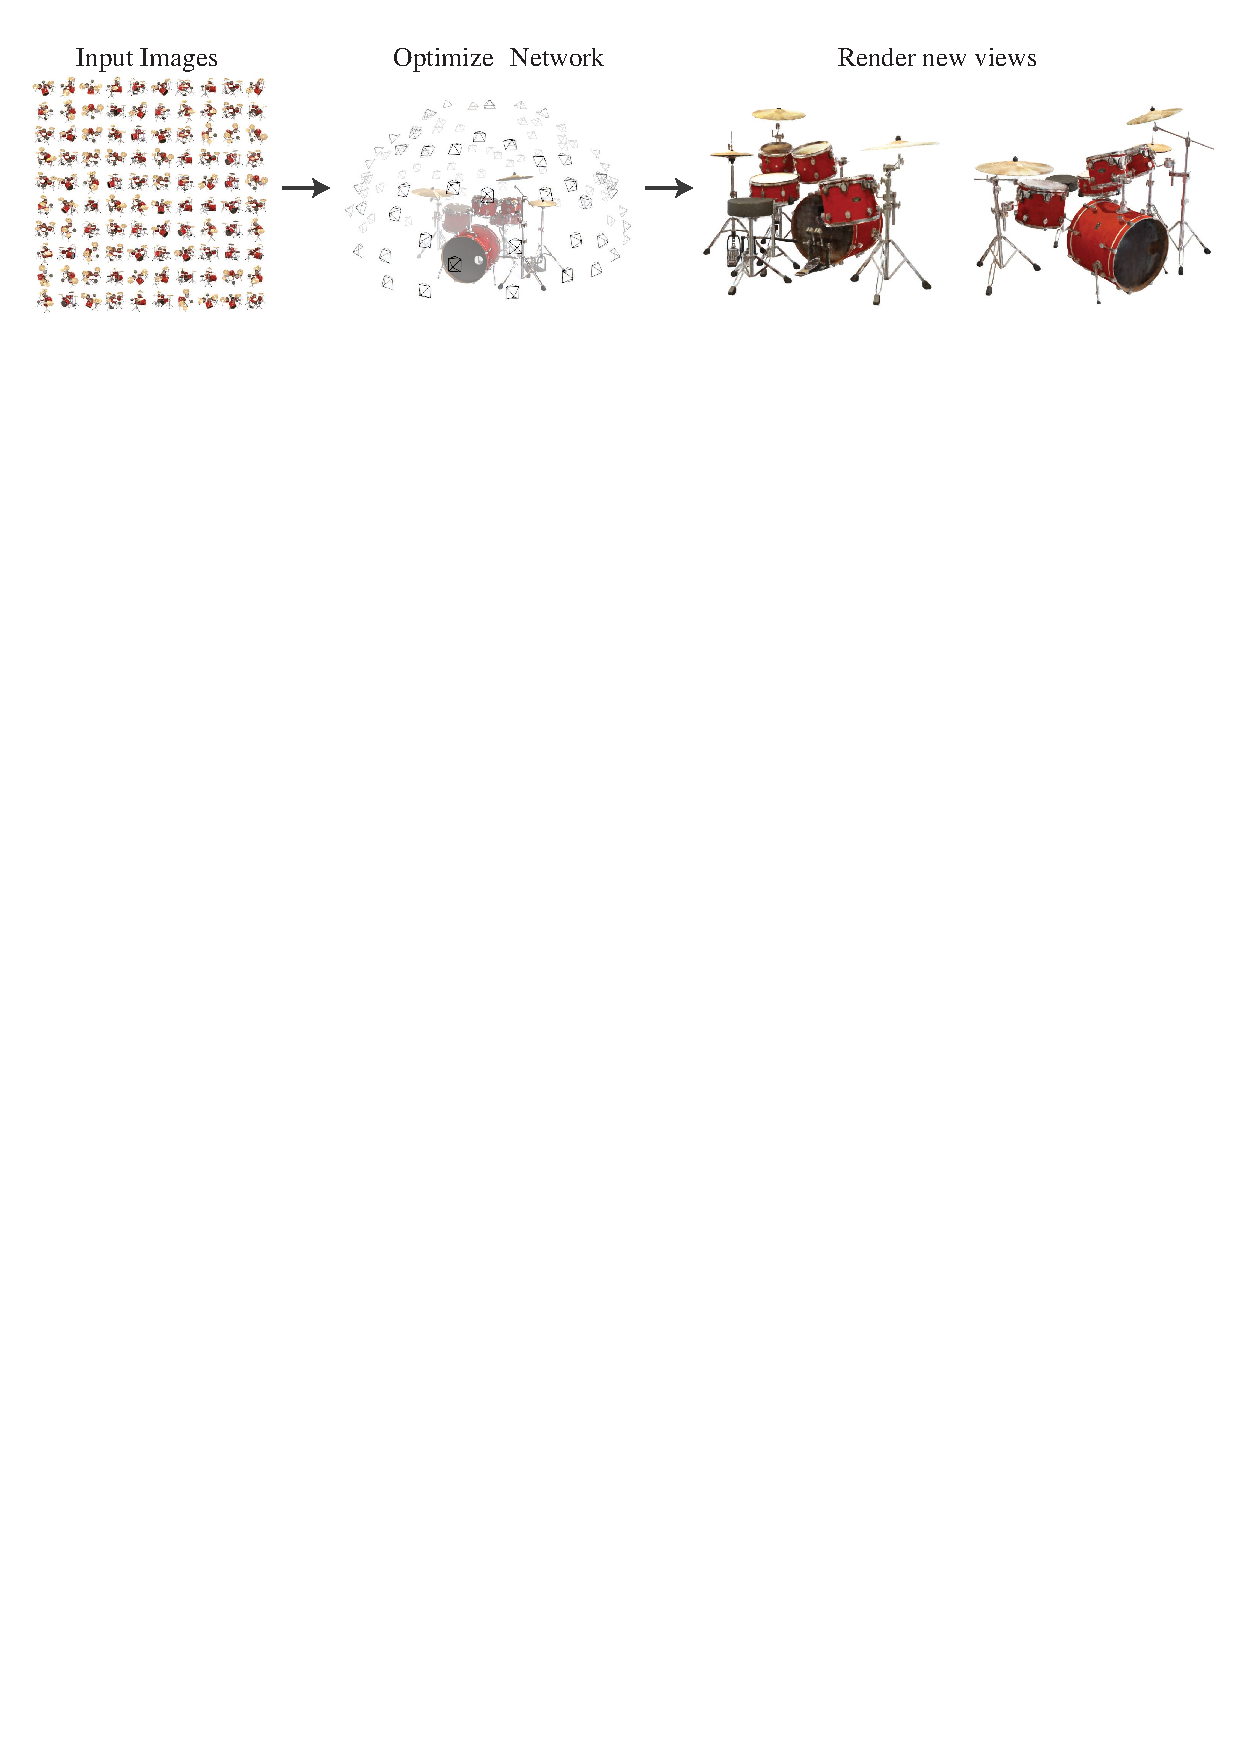
\includegraphics[width=0.95\linewidth]{figures/drums.pdf}
  \caption{新视角合成的过程\cite{mildenhall2020nerf}}
  \label{fig:novelviewsynthesis}
\end{figure}

\section{深度学习发展概述}
深度学习 (Deep Learning, DL) 是机器学习的一个分支,是一种以人工神经网络(如图~\ref{fig:neuralNetwork})为架构进行表征学习的方式。深度学习有着非常悠久的历史,最早可以追溯到20世纪40年代\cite{goodfellow2016deep}。学习可以是有监督的、无监督的,也可以是半监督的。

深度学习发展到现在,得益于 GPU 性能的巨大提升,已有诸如深度神经网络 (Deep Neural Network, DNN) ,深度置信网络\cite{hinton2009deep} (Deep Brief Network, DBN) ,循环神经网络\cite{rumelhart1986learning} (Recurrent Neural Network,RNN) ,卷积神经网络\cite{lecun1995convolutional} (Convolutional Neural Networks, CNN) 等深度学习网络模型已经服务于人工智能的各种领域。

由于本文主要涉及计算机视觉和计算机图形学的知识,因此接下来两小节会介绍这些领域最常用的两个网络架构,卷积神经网络和残差网络 Resnet 。

\begin{figure}[t]
  \centering
  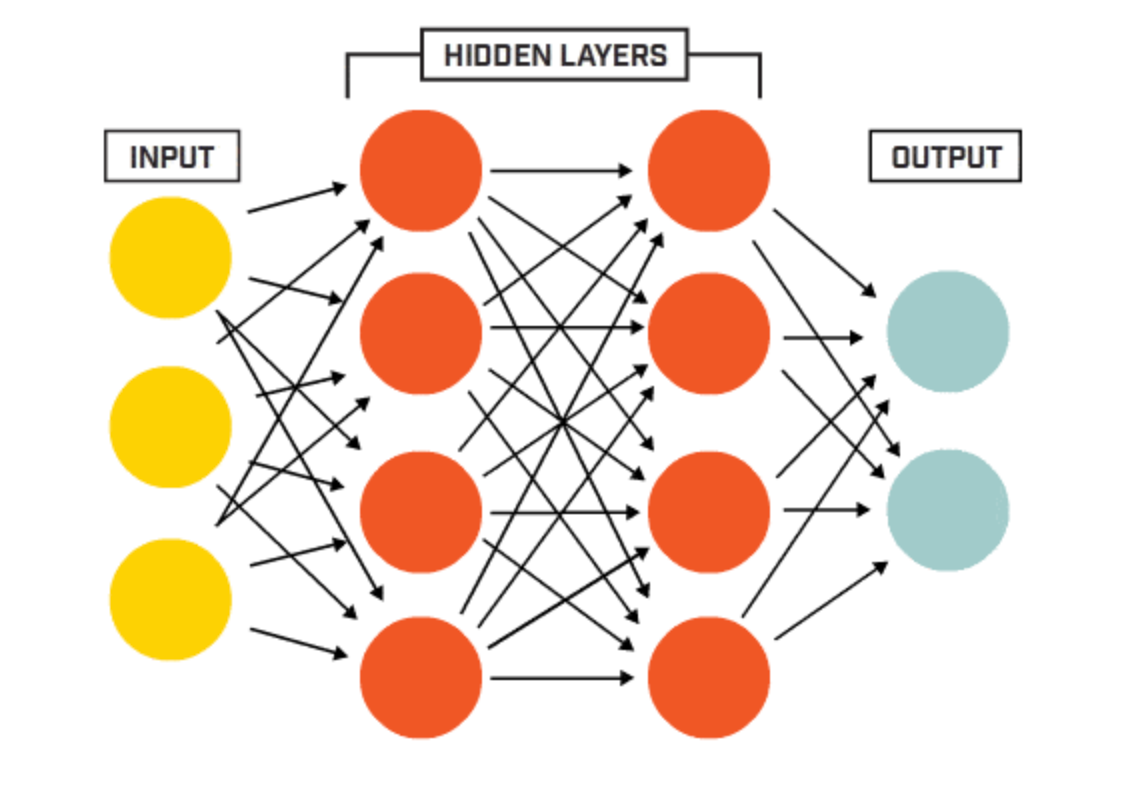
\includegraphics[width=0.9\linewidth]{figures/fc.png}
  \caption{神经网络示意图}
  \label{fig:neuralNetwork}
\end{figure}

\subsection{卷积神经网络}
要具体阐述卷积神经网络,就不得不先提到 MLP,如图~\ref{fig:neuralNetwork},一个最简单的 MLP 由三部分组成,包含基本的输入输出还有隐藏层。其中,隐藏层经常采用 sigmoid 和 tanh 作为激活函数。若不使用激活函数,即使是使用多层网络进行训练,实际上只相当于一层,只能进行简单的线性拟合,而有了激活函数网络则能够进行复杂的非线性拟合。不过在输入过大或者过小的时候,上述两种激活函数会出现梯度接近于0的情况,此时梯度更新幅度较小甚至是消失,神经网络的训练过程停滞。与 tanh 相比,sigmoid 还有个非常不利于学习的问题,那就是 sigmoid 函数的值域是$[0,1]$,也因此输出的均值不会为0,这非常不利于下一层的学习。为了解决上述问题,Glorot 等人\cite{glorot2011deep}提出了 ReLU 函数,解决了在输入为正数时梯度消失的问题,此外由于计算比 sigmoid 和 tanh 简单,前向传播和反向传播也都相应更快。

对于正向传播,$l$层的输出和$l-1$层的关系始终可以由下列公式来表达,而与网络深度无关。
\begin{equation}
    a^{l} = \sigma(z^{l}) = \sigma(f(a^{l-1})),
\end{equation}
其中$z^l = f(a^{l-1})$,$f$表示第$l$层网络对应的映射函数,$a^{l-1}$是前一层的输出(或第$l$层的输入),此外$\sigma$是激活函数。而反向传播则可用链式法则来进行每一层的求导,计算出梯度。

但是对于图像这种数据来说,全连接网络有着很大的问题,一方面,比如即便是$256 \times 256 \times 3$这样的小图像也需要数十万的参数,这么多参数会使得网络的训练难以进行下去;另一方面,图像数据不像其他任务中的数据,图像本身具有一定的高级语义,为了更好处理地处理像图像这样的二维数据,卷积神经网络应运而生。CNN 是一种前馈神经网络,除了全连接层,它还拥有着独有的卷积层,此外也会使用下采样的池化层。这一结构使得 CNN 对二维结构的数据(例如图像)进行很好的处理,当然训练过程也可以使用反向传播算法\cite{rumelhart1986learning}。由于存在着共享参数这一特性,卷积神经网络需要学习的参数比 MLP 更少,这使之成为深度学习领域影响力颇深的一种结构。

\begin{enumerate}
    \item 卷积层 \\
    实际上,卷积层是对输入进行特征提取的一种结构。卷积层一般会包含多个神经元,或者叫做卷积核,组成卷积核的每一个元素都会包含一个权重和一个偏移量 (Bias Vector)。卷积核在工作的时候会有规则的扫过输入的特征,对卷积核大小范围内的特征做矩阵乘法并求和,最后再叠加上偏移量。
    
    对一张二维图像$X$,卷积层的输出可表示为
    \begin{equation}
        y_{ij} = \sum_{u=1}^{m}\sum_{v=1}^{n}w_{uv} * x_{i-u+1,j-v+1},
    \end{equation}
    其中$x$表示输入图像$X\in{R^{M\times N}}$的一个像素大小,$w$是卷积核$W \in R^{m\times n}$的参数,一般地$m << M$,$n << N$。
    二维卷积的示意图如图~\ref{fig:2dconv}。
    \begin{figure}[htbp]
        \centering
        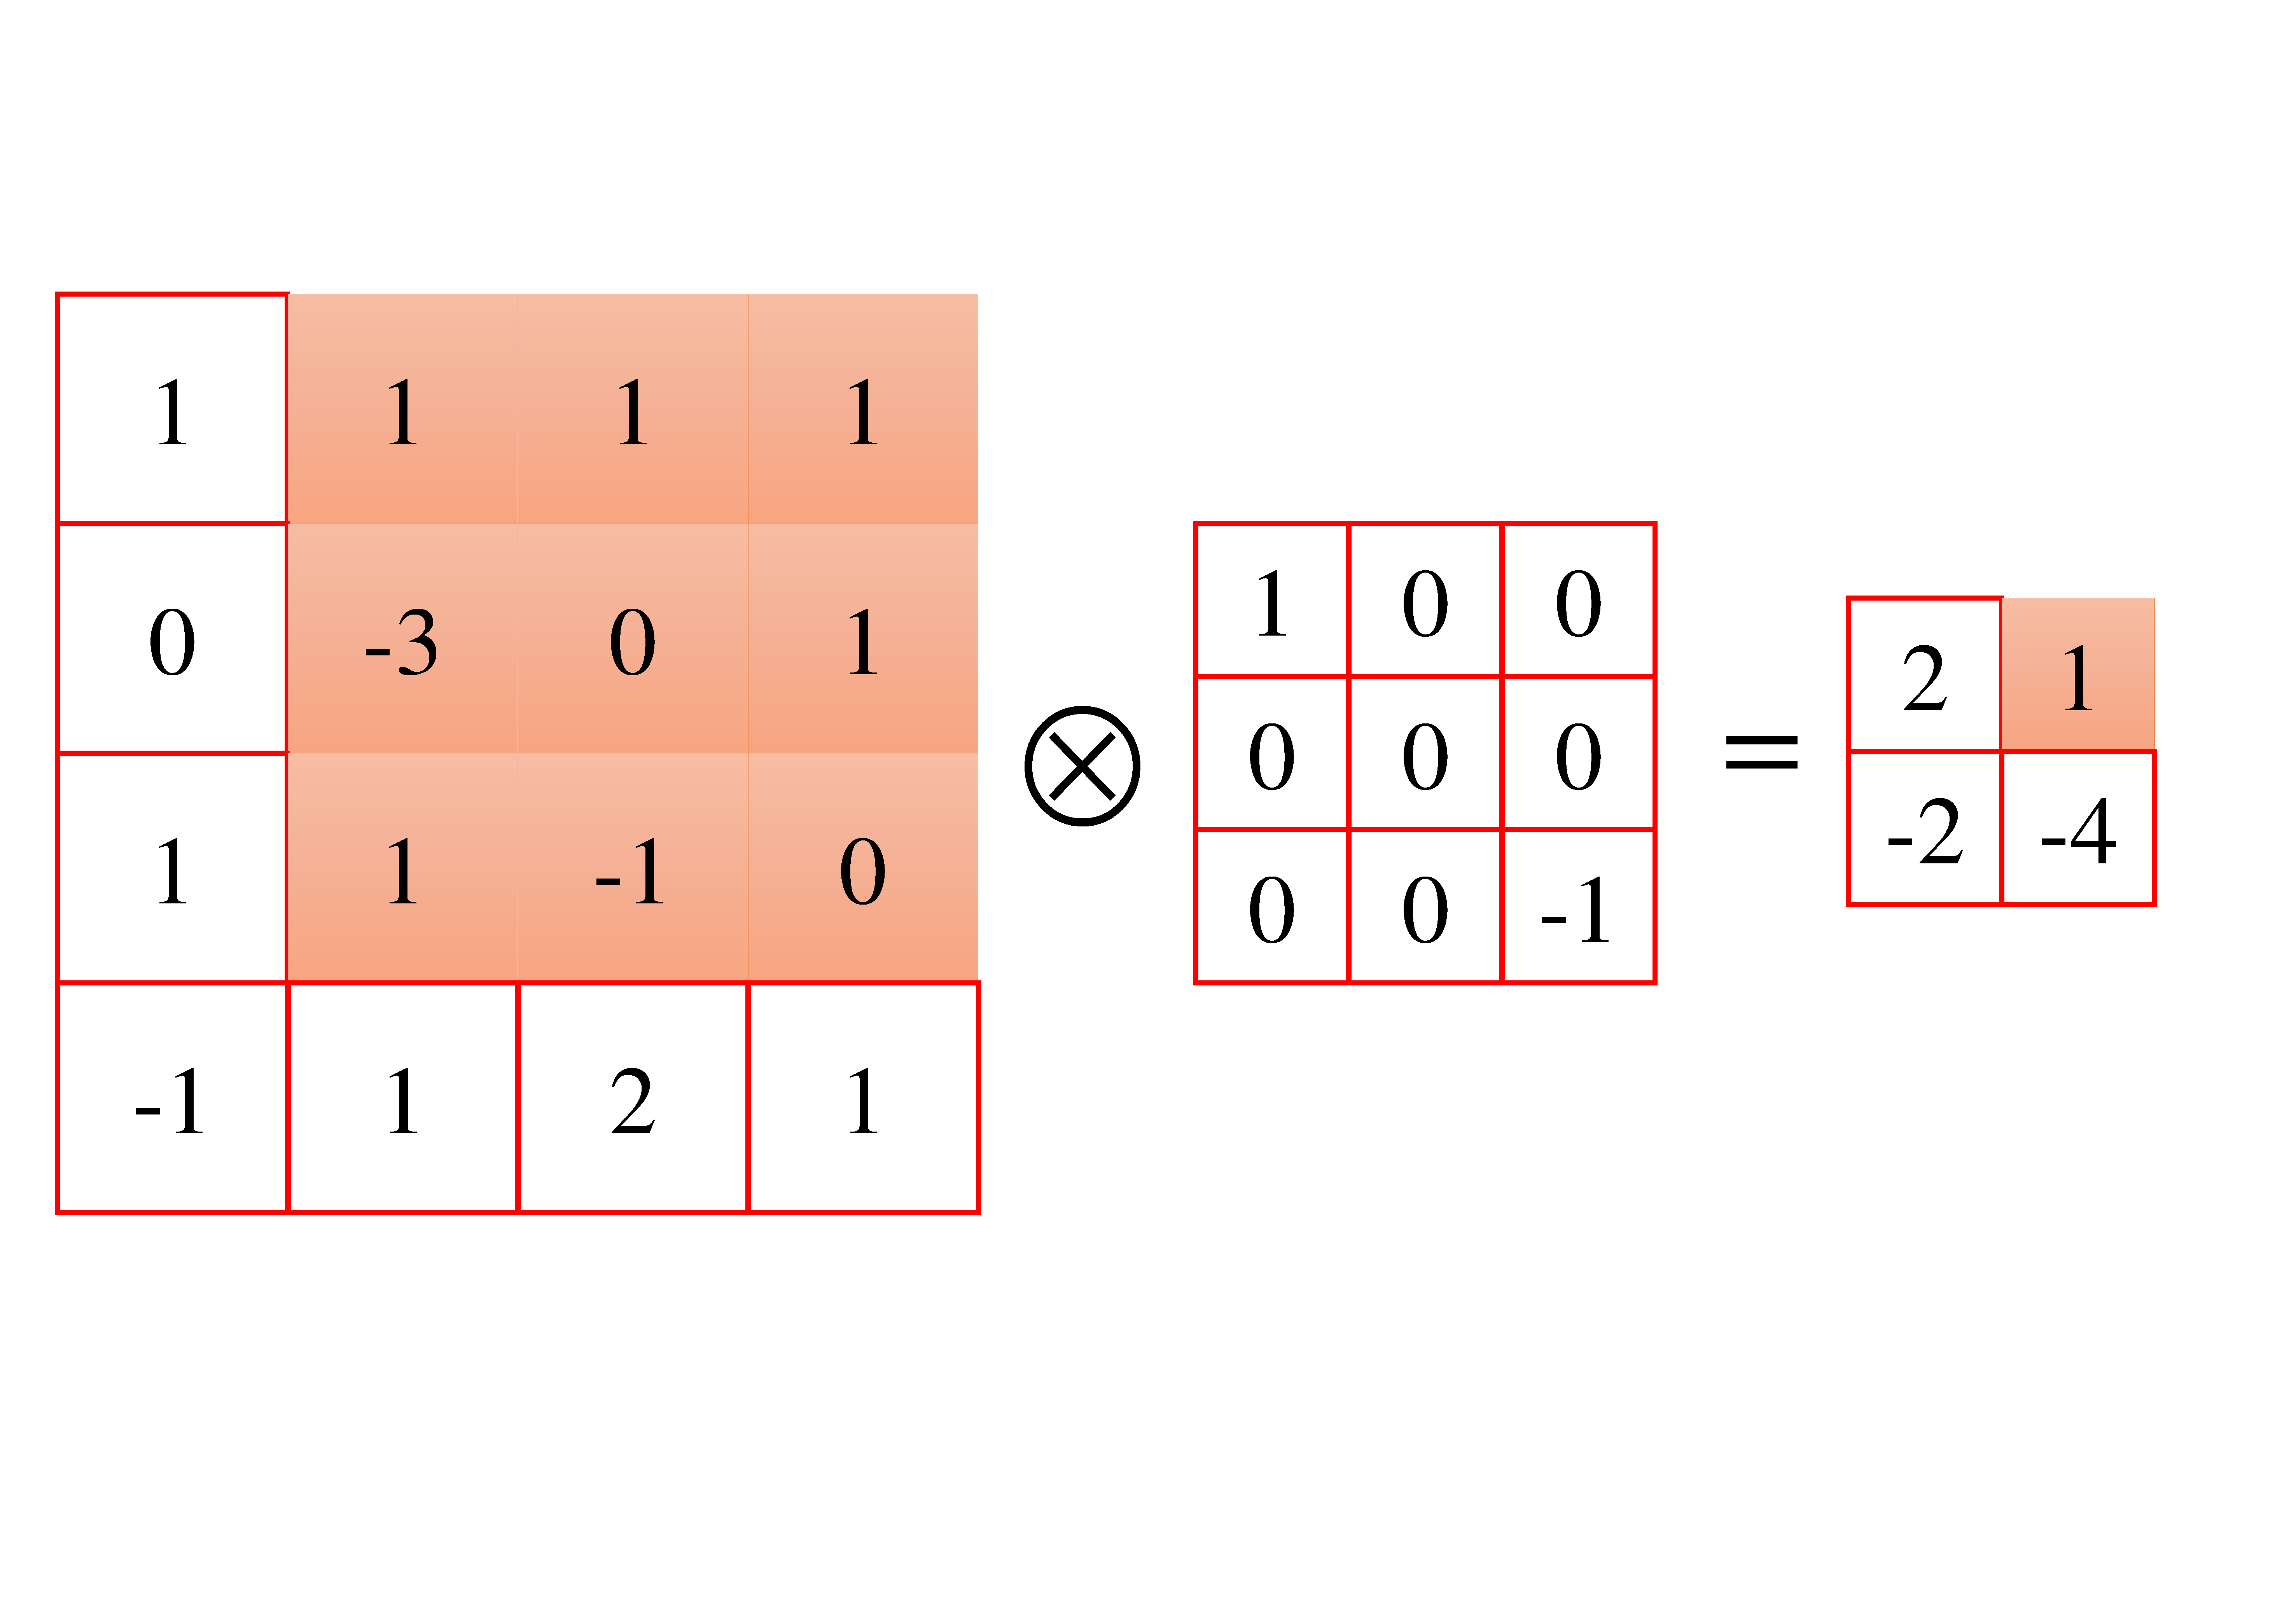
\includegraphics[width=0.7\linewidth]{figures/2dconv.pdf}
        \caption{二维卷积过程}
        \label{fig:2dconv}
    \end{figure}
    \item 池化层 \\
    池化层可以理解为下采样,减少输出特征的尺寸,能扩大感受野还能减少参数。最大池化和平均池化是最常见的两种方法。一般卷积层后会配合一个池化层,能进一步提取到有效的特征,保留主要特征并减少参数。
    \item 全连接层 \\
    无论说是一般的深度学习网络还是 CNN 这样稍微复杂的网络,全连接层都是关键所在。对于 MLP 这样的网络,那么就只有全连接层,可见全连接层的重要性。而对于卷积神经网络而言,全连接层就是将卷积层和池化层提取到的特征整合并输出预测结果。
\end{enumerate}

卷积层的提出极大地促进了计算机视觉领域的发展,AlexNet\cite{2012ImageNet} (5层卷积层、3层全连接层)在2012年的ImageNet视觉识别挑战赛中斩获冠军,可见CNN对于图像这样高级语义任务的巨大能力。此后,VGG\cite{simonyan2014very} 网络改进了 AlexNet 的网络,使得整个网络更深(19层),这使他成为了2014年 ImageNet 挑战赛的第一名。随着 VGG 的提出,人们开始倾向把网络加深,期望获得更好的识别效果。但实际上随着网络的逐渐加深,更深的网络难以训练,出现了因网络太深导致模型退化的问题,这是由于层数越深,训练误差越大,这与深度神经网络的初衷是背道而驰的,也不符合神经网络拟合任意复杂函数的理论。

但是众所周知的是,深度神经网络并没有消失在人们的视野里,这是由于残差网络 Resnet 的出现,这会在下一节进行具体介绍。
\subsection{残差网络 Resnet}
Kaiming He 等人借鉴了 Highway Network\cite{srivastava2015highway} 的跨层连接思想,并提出了赫赫有名的残差网络 Resnet\cite{he2016deep} ,较好地解决了当神经网络极深时模型失效无法训练的问题,并且在当时的 ImageNet 大赛上获得了第一名的好成绩。本文使用的神经辐射场的网络是基于残差模块设计的,因此接下来详细介绍残差网络的设计想法。

如图~\ref{fig:resnet} 所示,经典的残差网络由多个残差模块组成,因此可以根据需求自行设计网络的深度。残差网络核心思想是使用了 shortcut 这一操作,即将输入传到输出作为输出的一部分,用公式表达就是$H(x) = F(x) + x$,当$H(x) = x$时为恒等映射,这里的$F(x)$就是需要学习的残差。这样的设计原理是,当深度学习网络极深的时候,由于训练误差较大,无法提取出更抽象的特征,那么此时有了这样的残差结构,就可以学习到一个恒等映射,至少还能保留前面提取出的特征。虽然学习一个恒等映射不是非常容易,不过由于 shortcut 这一操作使得只需让残差往0的方向去学习即可,这样也同时有效避免了梯度消失的问题。resnet 的出现是具有划时代的意义的,它解决了极深的神经网络难以训练的问题,通过有效地学习到恒等映射来保证当网络越来越深的时候所导致的模型退化性能衰退的情况。

本文的基础网络架构就是引入了 skip connection(或者是上述的 shortcut )的操作来将输入的特征往网络深处传送,以此来训练出一个高质量的深度学习网络,这样才能学习到细粒度的连续的神经辐射场。

\begin{figure}[t]
    \centering
    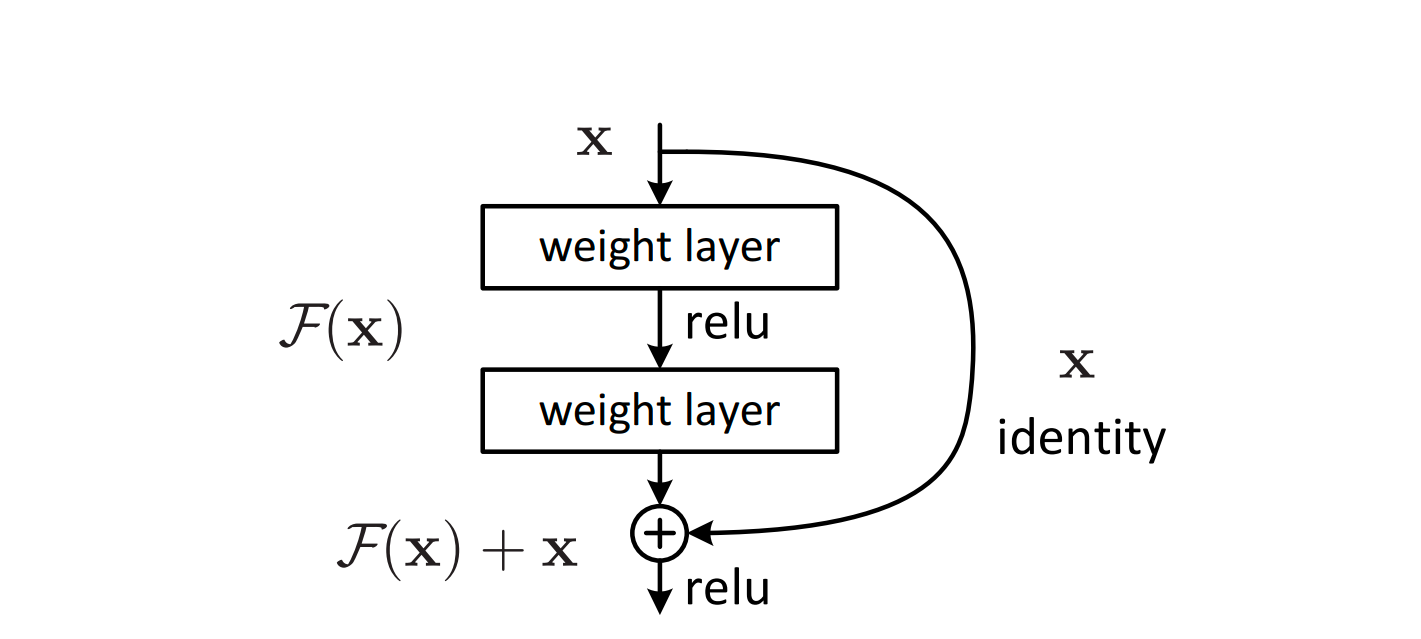
\includegraphics[width=0.7\linewidth]{figures/resnet.jpg}
    \caption{典型的残差结构}
    \label{fig:resnet}
\end{figure}

\section{查询表的加速方法}
在计算机科学中,查询表 (Lookup Table) 一般是一种简单的数组结构,通过简单的数组索引操作替代一些复杂的计算。一般来说,查询表的加速是很可观的,因为直接从内存中提取到相关数据往往要比复杂的计算快很多。

%一个经典的例子就是三角函数表。每次计算所需的正弦值在一些应用中可能会慢得无法忍受,为了避免这种情况,应用程序可以在刚开始的一段时间计算一定数量的角度的正弦值,譬如计算每个整数角度的正弦值,在后面的程序需要正弦值的时候,使用查找表从内存中提取临近角度的正弦值而不是使用数学公式进行计算。
一个典型的应用场景是自然对数表,在一些应用中,直接计算自然对数值是难以接受的,为了解决这一问题,可以提前将一些常用值的自然对数缓存在查询表中,在计算未知的对数值的时候,可以通过直接查询临近值的对数值而避免了复杂的数学计算,这大大加快了计算效率。

%一些折衷的方法是同时使用查找表和插值这样需要少许计算量的方法,这种方法对于两个预计算的值之间的部分能够提供更高的精度,这样稍微地增加了计算量但是大幅度地提高了应用程序所需的精度。根据预先计算的数值,这种方法在保持同样精度的前提下也减小了查找表的尺寸。

在一些细粒度的任务中,往往需要获得较高精度的查询结果,这时候就需要进行一些折衷,比如在使用查询表的同时结合插值的方法,通过略微增加计算量的方式增加了精度,同时也一定程度减少了查询表的尺寸。

%在图像处理中,查找表将索引号与输出值创建联系。颜色表作为一种普通的 LUT 是用来确定特定图像中每一像素所要显示的颜色和强度。

%另外需要注意的一个问题是,尽管查找表经常效率很高,但是如果所替换的计算相当简单的话就会得不偿失,这不仅仅因为从内存中提取结果需要更多的时间,而且因为它增大了所需的内存并且破坏了高速缓存。如果查找表太大,那么几乎每次访问查找表都会导致高速缓存缺失,这在处理器速度超过内存速度的时候愈发成为一个问题。
值得注意的是,虽然查询表的加速效率一般很高,但是通过查询表替换的计算方式过于简单,那么可能会出现从内存中提取数值的速度低于直接计算的速度,这样就得不偿失。

查询表实质是一种通过空间换时间的方式,但是实际应用中内存是有限的,因此必须要考虑查询表尺寸的问题。

%如何构建查找表有两个基本的约束条件,一个是可用内存的数量;不能构建一个超过能用内存空间的表格,尽管可以构建一个以查找速度为代价的基于磁盘的查找表。另外一个约束条件是初始计算查找表的时间——尽管这项工作不需要经常做,但是如果耗费的时间不可接受,那么也不适合使用查找表。

如图~\ref{fig:justlookup} 所示,以 justlookup\cite{lin2019justlookup} 为代表的工作拓宽了查询表的使用,justlookup 已经证明了对逐点网络可以去构建查询表来加速网络的前向传播并通过对近似特征再学习的策略来维持模型精度不损失,这一思想也可以应用到本文的模型加速上,通过查询表缓存网络参数,以此替换掉一些全连接层,这样可以少经过一些网络而直接通过查询表查询到中间层网络特征,从而加速前向传播。查询表技术在本文的具体应用详见下一章。

\begin{figure}[t]
    \centering
    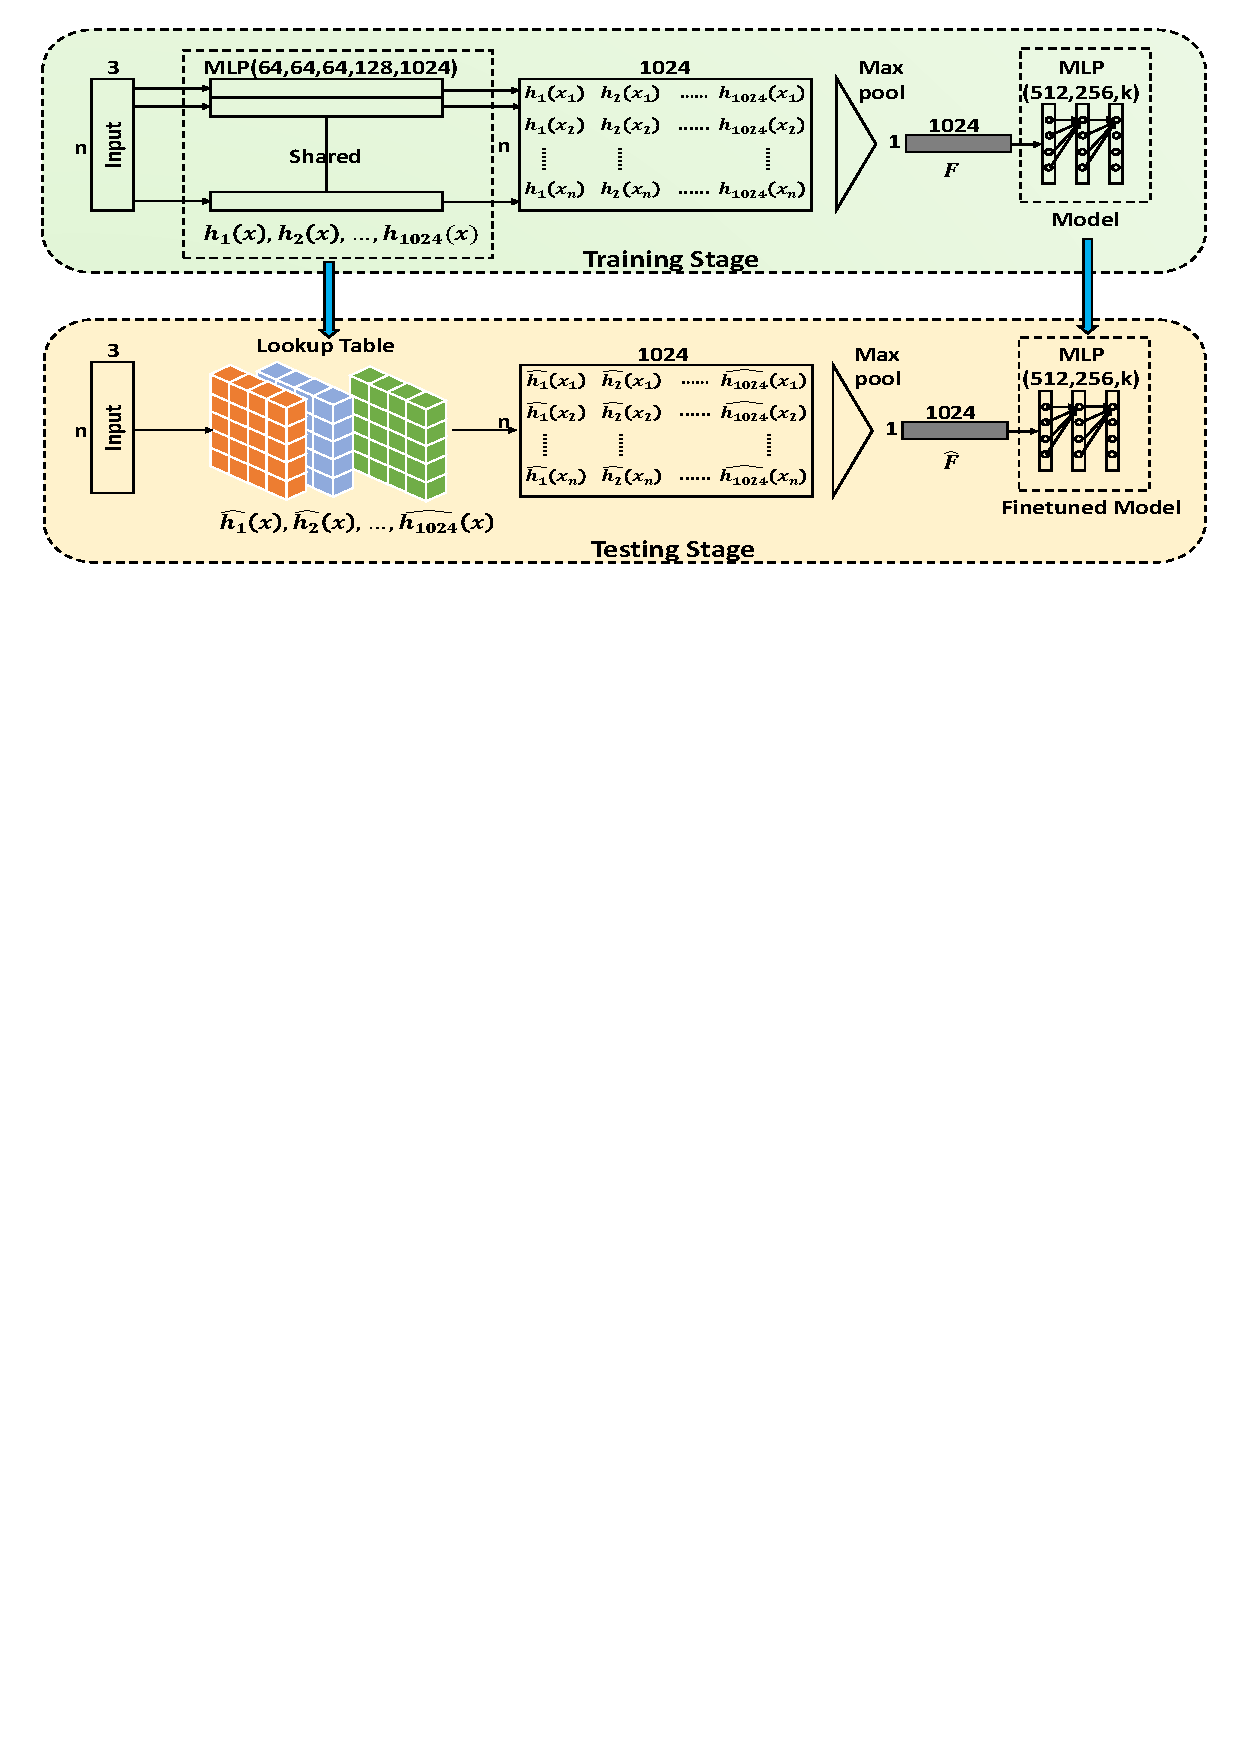
\includegraphics[width=0.9\linewidth]{figures/justlookup.pdf}
    \caption{查询表在逐点网络上的应用\cite{lin2019justlookup}}
    \label{fig:justlookup}
\end{figure}


\section{本章小结}
本章主要阐述了与本文系统相关的技术和理论方法,包含用于描述 3D 形状的一些表示方法,以及与本文任务最相关的新视图合成和基于图像的渲染,还有关于深度学习的一些基础概念,这些都构成了本文方法的基础。最后介绍了关于查询表的加速方法,以及将其应用到含有逐点网络的前向传播上的经典方法,这一思路也成为了本文方法的根基,将在下一章节详细阐述本文的方法。
